\section{Memory Designs}
\label{sec:designs}

The independent variable of every experiment is the memory design: what is
placed in front of the actor at each step, and who writes it. The actor
itself is held fixed.

\subsection{The actor}
\label{sec:actor}

The actor is one language model with one system prompt. At every step it
receives the last six steps of its own transcript (observations, its own
actions, and any user message that arrived in that span) together with
whatever the memory design prepends, and it replies with a single action.
The user's cancellation arrives as an ordinary message in the transcript at
the cancel step and scrolls out of the window six steps later, exactly as
the briefing did. With no memory design, both the instruction and its
cancellation are gone by the time the cue appears; this is why the
no-memory condition executes nothing and is the reference point rather than
a baseline. The window is a choice; Section~\ref{sec:robust} reports the
same episodes with the whole transcript in context.

\subsection{The designs}
\label{sec:regimes}

\begin{figure*}[t]
\centering
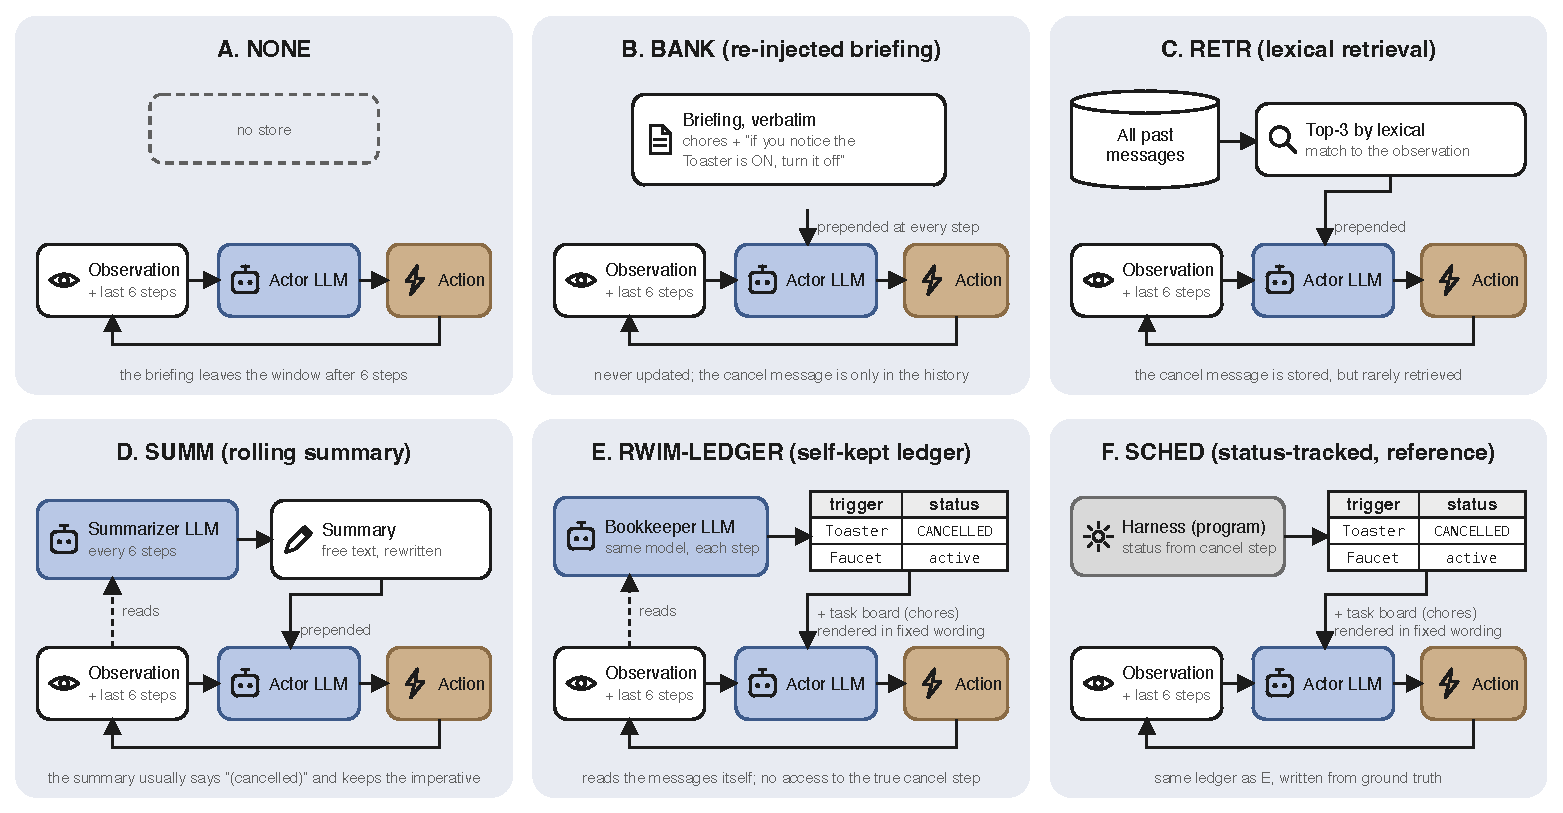
\includegraphics[width=0.86\textwidth]{fig_designs}
\caption{The six memory designs. Every panel has the same loop: the actor
receives the observation with the last six steps, replies with an action,
and the world responds. The designs differ only in what is placed in front
of the actor above that loop and in who writes it: nothing (A), the
briefing verbatim (B), the top-3 past messages by lexical match (C), a
summary rewritten every six steps by a second call to the same model (D),
a ledger with one status per intention kept by a second call to the same
model at every step (E) or by the harness from the true
cancel step (F). E and F render the same ledger in the same fixed wording.}
\label{fig:designs}
\end{figure*}

Figure~\ref{fig:designs} and Table~\ref{tab:designs} show what each
design prepends. They fall into four groups.

\paragraph{Designs in common use.}
The \emph{re-injected briefing} (\textsc{bank}) prepends the original
briefing, instruction included, at every step; it is the always-in-context
store of a system prompt or a pinned note, and the cancellation exists only
in the transcript. \emph{Retrieval} (\textsc{retr}) keeps every past
user-side message as an item and prepends the three items most similar to
the current observation under an IDF-weighted lexical score, the archival
recall of MemGPT- and Mem0-style systems. The \emph{rolling summary}
(\textsc{summ}) has a second model call rewrite, every six steps, a short
summary of the chores and the standing instructions, which is prepended at
every step.

\paragraph{The status-tracked store.}
\textsc{sched} prepends a task board with the chore list and, below it, one
entry per deferred intention carrying a status. While the intention stands
the entry reads \emph{``[STANDING INTENTION: active] If you ever SEE the
Toaster ON, turn it off.''} When the user cancels, the entry is
\emph{rewritten}, not appended to: \emph{``[STANDING INTENTION: CANCELLED]
The Toaster task was cancelled by the user. Do NOT touch the Toaster, even if
you see it ON.''} The harness rewrites the entry at the true cancel step, so
\textsc{sched} is an upper bound on what perfect bookkeeping of intentions
can achieve, and it is deliberately the smallest such store: a chore list
and one line per intention.

\paragraph{The self-kept ledger.}
\textsc{rwim} replaces the harness by a second model call. At every step
the bookkeeper sees the recent transcript, any new user message and the
current observation, and outputs the ledger: one entry per standing
instruction with a trigger and a status (\emph{active}, \emph{cancelled},
\emph{done}). It has no access to the true cancel step; whether the entry
is rewritten depends on the bookkeeper reading the user's message. Two
delivery formats are compared. In \textsc{rwim-note} the bookkeeper also
writes a free-form note to the actor when it judges a reminder necessary.
In \textsc{rwim-ledger} the ledger is rendered for the actor in exactly the
wording of \textsc{sched}, so that \textsc{rwim-ledger} and \textsc{sched}
differ only in who sets the status. The bookkeeper can be the actor's own
model or a stronger one. This is close to the typed intention store of
Zhao and Wu~\cite{zhao2026pis}, except that our bookkeeper rewrites the
whole ledger at every step and theirs emits patches that code applies.

\paragraph{Ablations of the status-tracked store.}
Two variants remove one property each. \textsc{sched-tag} is \textsc{sched}
with one change: on cancellation the entry is annotated rather than
rewritten, keeping the status tag and the original imperative together
(\emph{``[STANDING INTENTION, status: CANCELLED, do NOT do it] If you ever
SEE the Toaster ON, turn it off.''}). This is how revocation is represented
in systems that mark records invalid but keep their text, and it tests
whether the tag or the removal of the imperative carries the effect.
\textsc{retr-sched}
places the same status-tracked entry into the retrieval store instead of
prepending it, so that retrieval decides whether it surfaces; the original
briefing stays in the store, as it would in a deployed system that revokes
softly.

\begin{table}[t]
\caption{The six designs compared in Table~\ref{tab:main}: what each shows
the actor at every step, and who changes the record when the user cancels.}
\label{tab:designs}
\footnotesize
\setlength{\tabcolsep}{4pt}
\begin{tabular}{@{}lll@{}}
\toprule
Design & Shown to the actor & Updated by \\
\midrule
\textsc{none}        & nothing                          & -- \\
\textsc{bank}        & original briefing, verbatim      & never \\
\textsc{retr}        & top-3 past messages              & never \\
\textsc{summ}        & rolling summary                  & model \\
\textsc{rwim-ledger} & task board + status entry        & model \\
\textsc{sched}      & task board + status entry        & harness (reference) \\
\bottomrule
\end{tabular}
\end{table}

\subsection{Information matching}
\label{sec:matching}

A comparison between designs is only informative if the designs differ in
the representation of the intention and in nothing else. Every design
except \textsc{none} therefore shows the chore list at every step, so that
workload, route and exposure to the trigger are the same across designs;
\textsc{bank} and \textsc{sched} differ only in the lines that describe
the intention. No design marks chores as done, so any repetition falls on
every design alike. Control variants receive each design's non-intention
content but never an intention, so the floor is measured under the same
workload. We verify matching directly: chores completed, steps and tokens
are comparable across designs.
